\documentclass[10pt]{amsart}
\usepackage{amssymb}
\usepackage[margin=1in]{geometry}
\usepackage{tikz}

\newcommand{\Card}{\operatorname{Card}}

\begin{document}
\author{Ignat Soroko}
\title{A brief description of the functionality of the accompanying code}
\maketitle

\noindent
The file {\tt hindex.g} accompanies the paper
\begin{quote}
``Divergence, thickness and hypergraph index for general Coxeter groups'' by Pallavi Dani, Yusra Naqvi, Ignat Soroko and Anne Thomas
\end{quote}
and contains some code for the computer algebra system {\tt GAP4} for computing:
\begin{itemize}
\item the hypergraph index
\item the duplex construction
\item the number of ends of the Coxeter group
\item some Coxeter matrices used in the text.
\end{itemize}

\bigskip

\section{A typical {\tt GAP} session}

{\footnotesize
\begin{verbatim}
gap> Read("hindex.g");
gap> m3:=DaniThomasGamma(3);
[ [ 1, 0, 2, 2, 2, 2, 0, 0 ], [ 0, 1, 2, 2, 2, 2, 0, 0 ], [ 2, 2, 1, 0, 0, 0, 2, 0 ], [ 2, 2, 0, 1, 0, 0, 2, 0 ], 
  [ 2, 2, 0, 0, 1, 0, 0, 2 ], [ 2, 2, 0, 0, 0, 1, 0, 0 ], [ 0, 0, 2, 2, 0, 0, 1, 2 ], [ 0, 0, 0, 0, 2, 0, 2, 1 ] ]
gap> h3:=HypergraphIndex(m3);
[ 2, [ [ [ 1, 2, 3, 4, 5, 6 ], [ 1, 2, 3, 4, 7 ], [ 1, 5, 8 ], [ 2, 5, 8 ], [ 3, 7, 8 ], [ 4, 7, 8 ], [ 5, 7, 8 ] ], 
      [ [ 1 .. 7 ], [ 1, 5, 8 ], [ 2, 5, 8 ], [ 3, 7, 8 ], [ 4, 7, 8 ], [ 5, 7, 8 ] ], 
      [ [ 1 .. 8 ], [ 1, 5, 8 ], [ 2, 5, 8 ], [ 3, 7, 8 ], [ 4, 7, 8 ] ] ] ] 
\end{verbatim}
}

\bigskip\noindent
Here the command 
{\footnotesize
\begin{verbatim}
gap> Read("hindex.g");
\end{verbatim}}\noindent
loads the file {\tt hindex.g}, and it needs to be done just once.

\medskip\noindent
{\footnotesize
\begin{verbatim}
gap> m3:=DaniThomasGamma(3);
\end{verbatim}}

\noindent
loads the Coxeter matrix of the right-angled Coxeter group $\Gamma_3$, whose {\it defining graph\/} is depicted below (see also Figure~5 of the article). Note that, by our convention, in a Coxeter matrix {\tt0} represents infinity. The numeration of vertices in the Coxeter matrix for $\Gamma_3$ is as follows:

\begin{figure}[htb!] 
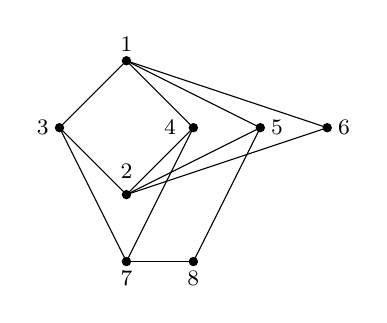
\begin{tikzpicture}[scale=0.85]
\fill (0,1) circle (2pt); \draw (0,1.25) node {\footnotesize $1$};
\fill (0,-1) circle (2pt); \draw (0,-0.65) node {\footnotesize $2$};
\fill (0,-2) circle (2pt); \draw (0,-2.25) node {\footnotesize $7$};
\fill (1,-2) circle (2pt); \draw (1,-2.25) node {\footnotesize $8$};
\fill (-1,0) circle (2pt); \draw (-1.25,0) node {\footnotesize $3$};
\fill (1,0) circle (2pt); \draw (0.65,0) node {\footnotesize $4$};
\fill (2,0) circle (2pt); \draw (2.25,0) node {\footnotesize $5$};
\fill (3,0) circle (2pt); \draw (3.25,0) node {\footnotesize $6$};
\draw (-1,0)--(0,1);
\draw (-1,0)--(0,-1);
\draw (-1,0)--(0,-2);
\draw (1,0)--(0,1);
\draw (1,0)--(0,-1);
\draw (1,0)--(0,-2);
\draw (2,0)--(0,1);
\draw (2,0)--(0,-1);
\draw (3,0)--(0,1);
\draw (3,0)--(0,-1);
\draw (1,-2)--(0,-2);
\draw (1,-2)--(2,0);
\end{tikzpicture}
\end{figure}

\noindent
Recall that in the defining graph an edge corresponds to a pair of commuting generators $s,t$, i.e.\ such that $m_{st}=2$, and no edge between $s,t$ corresponds to $m_{st}=\infty$.

\medskip\noindent
{\footnotesize
\begin{verbatim}
gap> h3:=HypergraphIndex(m3);
\end{verbatim}}\noindent
returns a list of length two. Its first component, {\tt 2}, is the hypergraph index $h$ of the corresponding Coxeter system. The second component is the list $[\Lambda_0,\Lambda_1,\dots,\Lambda_h]$, where each sublist $\Lambda_i$ is a list of lists of integers, which represent subsets of the generating set. I.e. $\Lambda_0$ is
\medskip\noindent
{\footnotesize
\begin{verbatim}
[ [ 1, 2, 3, 4, 5, 6 ], [ 1, 2, 3, 4, 7 ], [ 1, 5, 8 ], [ 2, 5, 8 ], [ 3, 7, 8 ], [ 4, 7, 8 ], [ 5, 7, 8 ] ]
\end{verbatim}}

\noindent
which means that $\Lambda_0$ contains wide subsets $\{1,2\}\times\{3,4,5,6\}$ and $\{3,4\}\times\{1,2,7\}$ and slab subsets $\{1,8\}\times\{5\}$, $\{2,8\}\times\{5\}$, $\{3,8\}\times\{7\}$, $\{4,8\}\times\{7\}$, and $\{5,7\}\times\{8\}$. Moreover, we see that the two wide subsets intersect in a nonspherical system $\{1,2\}\times\{3,4\}$, so they should be united in $\Lambda_1$, which is equal to the second entry in the list discussed above:
\medskip\noindent
{\footnotesize
\begin{verbatim}
[ [ 1 .. 7 ], [ 1, 5, 8 ], [ 2, 5, 8 ], [ 3, 7, 8 ], [ 4, 7, 8 ], [ 5, 7, 8 ] ]
\end{verbatim}}\noindent
And finally we see that the elements $\{1,\dots,7\}$ and $\{5,7\}\times\{8\}$ in $\Lambda_1$ intersect in a nonspherical subsystem $\{5,7\}$, and hence should be united in $\Lambda_2$. Thus $\Lambda_2$ contains the whole generator set $\{1,\dots,8\}$, which is represented by the third entry in the above list: $\Lambda_2$ equals
\medskip\noindent
{\footnotesize
\begin{verbatim}
[ [ 1 .. 8 ], [ 1, 5, 8 ], [ 2, 5, 8 ], [ 3, 7, 8 ], [ 4, 7, 8 ] ] 
\end{verbatim}}\noindent
Since the whole generator set {\tt [ 1 .. 8 ]} belongs to $\Lambda_2$, the hypergraph index $h$ is equal to 2.


\section{Main functions}

\noindent
{\tt $\blacktriangleright$ HypergraphIndex(mat)}

\noindent 
\begin{itemize}
\item{} Input: A Coxeter matrix {\tt mat}.
\item{} Output: A list {\tt [hi,L]} of length two:
\begin{itemize}
\item{} {\tt hi} is the hypergraph index, which is an integer {\tt 0,1,2,\dots} or {\tt infinity}.
\item{} {\tt L} is the list of lists which represents sets $[\Lambda_0,\Lambda_1,\dots,\Lambda_h]$.
\end{itemize}
\end{itemize}
%\noindent
Each $\Lambda_i$ is a list of lists of integers corresponding to the subsets of the generating set $S$, which is identified with {\tt [1..N]} for $\mathtt{N}=\Card(S)$, see the example above.

\subsection*{Remark} To speed up computations, we form the slab subsets $\Psi(S)$ in a modified form. Instead of subsets $A\times K$ where $A\subset S$ is minimal nonspherical and $K\subset S$ is a spherical subset commuting with $A$, such that $A\times K$ have maximality property as per Definition~4.5 of the article, we store subsets of the form $A\times\{s\}$ where $A$ is as before, and $s$ commutes with $A$. This makes $\Lambda_0$ different from the one defined in the article, however this has no bearing on the sets $\Lambda_1,\Lambda_2,\dots$ and they are exactly as they should be.

\bigskip\noindent
{\tt $\blacktriangleright$ DuplexRACG(mat,m,n)}
\noindent 
\begin{itemize}
\item{} Input: 
	\begin{itemize}
	\item A Coxeter matrix {\tt mat} of a right-angled Coxeter system;
	\item {\tt m,n} are two integers $\ge 2$ or $0$ (which represents $\infty$).
	\end{itemize}
\item{} Output: the Coxeter matrix corresponding to the duplex construction as described in Section~5 of the article.
\end{itemize}



\section{Functions to form Coxeter matrices}

\noindent
{\tt $\blacktriangleright$ CoxeterMatrixDynkinPath(lst)}
\noindent 
\begin{itemize}
\item{} Input: a list {\tt lst} of edge labels corresponding to the Dynkin diagram which is a simple path.
\item{} Output: the Coxeter matrix of the corresponding Coxeter system.
\item Example: 

\noindent
\verb+gap> mEx9:=CoxeterMatrixDynkinPath([4,4,4,4,4,4,4]);+

\noindent
creates the Coxeter matrix of the Coxeter system $\Delta_8$ depicted in Figure~9 of the article.
\end{itemize}

\bigskip
\noindent
{\tt $\blacktriangleright$ CoxeterMatrixDynkinCycle(lst)}
\noindent 
\begin{itemize}
\item{} Input: a list {\tt lst} of edge labels corresponding to the Dynkin diagram which is a simple cycle.
\item{} Output: the Coxeter matrix of the corresponding Coxeter system.
\item Examples: 

\noindent
\verb+gap> mEx10a:=CoxeterMatrixDynkinCycle([3,3,3,3,3,3,3,3,3]);+

\noindent
\verb+gap> mEx10b:=CoxeterMatrixDynkinCycle([4,3,3,4,4,4,3,3,4]);+

\noindent
\verb+gap> mEx10c:=CoxeterMatrixDynkinCycle([3,4,4,3,3,3,4,4,3]);+

\noindent
\verb+gap> mEx10d:=CoxeterMatrixDynkinCycle([4,3,4,4,3,4,4,3,4]);+

\noindent
create the Coxeter matrices of the Coxeter systems depicted in Figure~10 of the article.
\end{itemize}



\bigskip
\noindent
{\tt $\blacktriangleright$ CoxeterMatrixRAListOfEdges(edges)}
\noindent 
\begin{itemize}
\item{} Input: a list of pairs of integers representing edges of the defining graph of a right-angled Coxeter system;
\item{} Output: the Coxeter matrix of the corresponding right-angled Coxeter system.
\end{itemize}

\bigskip
\noindent
Besides, the constructors of Coxeter matrices for irreducible spherical and affine and Coxeter systems are provided, as well as for the two Lann\'er hyperbolic systems which are not paths or cycles.

\bigskip\noindent
{\tt
\begin{tabular}{l@{\qquad}l}
CoxeterMatrixAn(n)& CoxeterMatrixAffineAn\char`_(n)\\
CoxeterMatrixBn(n)& CoxeterMatrixAffineBn\char`_(n)\\
CoxeterMatrixCn(n) {(\rm same as the above)}& CoxeterMatrixAffineCn\char`_(n)\\
CoxeterMatrixDn(n)& CoxeterMatrixAffineDn\char`_(n)\\
CoxeterMatrixEn(n) {\rm($\mathtt n=6,7,8$, vertex 4 is branch)}& CoxeterMatrixAffineEn\char`_(n)\\
CoxeterMatrixFn(n) {\rm($\mathtt n=4$)}& CoxeterMatrixAffineFn\char`_(n)\\
CoxeterMatrixGn(n) {\rm($\mathtt n=2$)} & CoxeterMatrixAffineGn\char`_(n)\\
CoxeterMatrixHn(n) {\rm($\mathtt n=2,3,4$; $m_{12}=5$)}&\\
CoxeterMatrixI2m(m) {\rm($\mathtt m\ne1$)} & CoxeterMatrixLannerZn(n) {\rm($\mathtt n=4,5$)}
\end{tabular}
}

\bigskip
\noindent
Here for all systems (including affine ones) the argument $\mathtt n$ is the number of vertices. For the function {\tt CoxeterMatrixI2m(m)} the argument {\tt m} is the edge label between the two vertices.


\bigskip
\noindent
Other Coxeter matrices provided in the file {\tt hindex.g}:

\bigskip
\noindent
{\tt $\blacktriangleright$ DaniThomasGamma(d)}
\noindent 
\begin{itemize}
\item{} Input: An integer {\tt d}
\item{} Output: The Coxeter matrix of the right-angled Coxeter system $\Gamma_d$ from the article of Dani and Thomas, which are also depicted in Figure~6 of the main paper.
\end{itemize}


\bigskip
\noindent
{\tt $\blacktriangleright$ mEx4, mEx9, mEx10a, mEx10b, mEx10c, mEx10d, mEx11}

\noindent
provide Coxeter matrices for the systems presented in the Figures 4, 9, 10a--d, and 11 of the article.

\bigskip
\noindent
{\tt $\blacktriangleright$ CoxeterSubmatrix(mat,T)}
\noindent 
\begin{itemize}
\item{} Input: a Coxeter matrix {\tt mat} and a subset {\tt T} of {\tt [1..Size(mat)]}
\item{} Output: the Coxeter matrix corresponding to the subsystem on the set of vertices {\tt T}.
\end{itemize}




\bigskip
\section{Other useful functions}

\noindent
{\tt $\blacktriangleright$ IsOneEnded(mat)}
\noindent 
\begin{itemize}
\item{} Input: A Coxeter matrix {\tt mat};
\item{} Output: {\tt true} or {\tt false} depending on whether the Coxeter group with the Coxeter matrix {\tt mat} has one end. Uses the criterion from Th.~8.7.2 of the Davis's book.
\end{itemize}

\bigskip\noindent
{\tt $\blacktriangleright$ NrEnds(mat)}
\noindent 
\begin{itemize}
\item{} Input: A Coxeter matrix {\tt mat};
\item{} Output: an integer {\tt 0,1,2} or {\tt infinity} representing the number of ends of the corresponding Coxeter group. Uses Theorems~8.7.2, 8.7.3 and 8.7.4 of the Davis's book.
\end{itemize}

\bigskip\noindent
{\tt $\blacktriangleright$ CanonicalRepOrbit(mat)}
\noindent 
\begin{itemize}
\item{} Input: A Coxeter matrix {\tt mat};
\item{} Output: A permuted Coxeter matrix, which is a canonical representative under the action of all permutations of the Coxeter generating set. 
\end{itemize}
\noindent It returns the Coxeter matrix which is maximal in the lexicographic order for all simultaneous permutations of rows and columns applied to {\tt mat}. It first computes the vector of sums of edge labels at each vertex, sorts the resulting vector in the descending order, and then applies only those permutations that preserve this vector. This function is useful when comparing Coxeter systems up to isomorphism of edge-labeled graphs. 



\bigskip\bigskip
\section{Support}
\noindent
For anything related to the code it is best to contact Ignat Soroko by email {\tt ignat.soroko@gmail.com}.

\end{document}